\documentclass[a4paper,11pt]{article}
\usepackage[utf8]{inputenc}
\usepackage[MeX]{polski}
\usepackage{hyperref}
\usepackage{graphicx}
\usepackage{pdfpages}
\usepackage{tikz}
\usepackage{fancyvrb}
\usepackage{rotating}
\usepackage{multirow}
\usetikzlibrary{positioning,shapes,shadows,arrows}

\author{Michał Aniserowicz \href{mailto:michalaniserowicz@gmail.com}{{\small \nolinkurl{<michalaniserowicz@gmail.com>}}} \\ Jakub Turek \href{mailto:jkbturek@gmail.com}{{\small \nolinkurl{jkbturek@gmail.com}}}}
\title{{\Large [WEDT.A] Dokumentacja końcowa projektu} \\ Klasyfikacja stron WWW na podstawie struktury}
\date{30 maja 2013r.}

\begin{document}

\maketitle

\section{Temat projektu}

Tematem projektu jest automatyczna klasyfikacja stron WWW na podstawie struktury. W~ramach uścieślenia tematu projektu, wybrane do rozpoznowania zostały następujące kategorie stron internetowych:

\begin{itemize}
 \item dzienniki internetowe (\emph{blogi}),
 \item strony społecznościowe oparte na obrazkach (\emph{kwejki}),
 \item serwisy informacyjne,
 \item sklepy internetowe.
\end{itemize}

Projekt został wykonany w technologii Python 2.7.4 i~był testowany na systemach operacyjnych Windows~7 oraz Ubuntu~13.04. Projekt wykorzystuje bibliotekę PIL\footnote{Python Image Library - \href{http://www.pythonware.com/products/pil/}{http://www.pythonware.com/products/pil/}.} w~wersji 1.1.7.

\section{Implementacja}

\subsection{Schemat działania aplikacji}

Na następnej stronie przedstawiony został ogólny schemat działania programu. Obejmuje on dwie główne fazy działania aplikacji:

\begin{description}
    \item[uczenie się] Program generuje zestawienie wartości cech dla poszczególnych kategorii na podstawie próby wzorców.
    \item[klasyfikacja] Program dokonuje klasyfikacji pozostałych stron na podstawie wartości cech wyznaczonych w~poprzednim kroku.
\end{description}

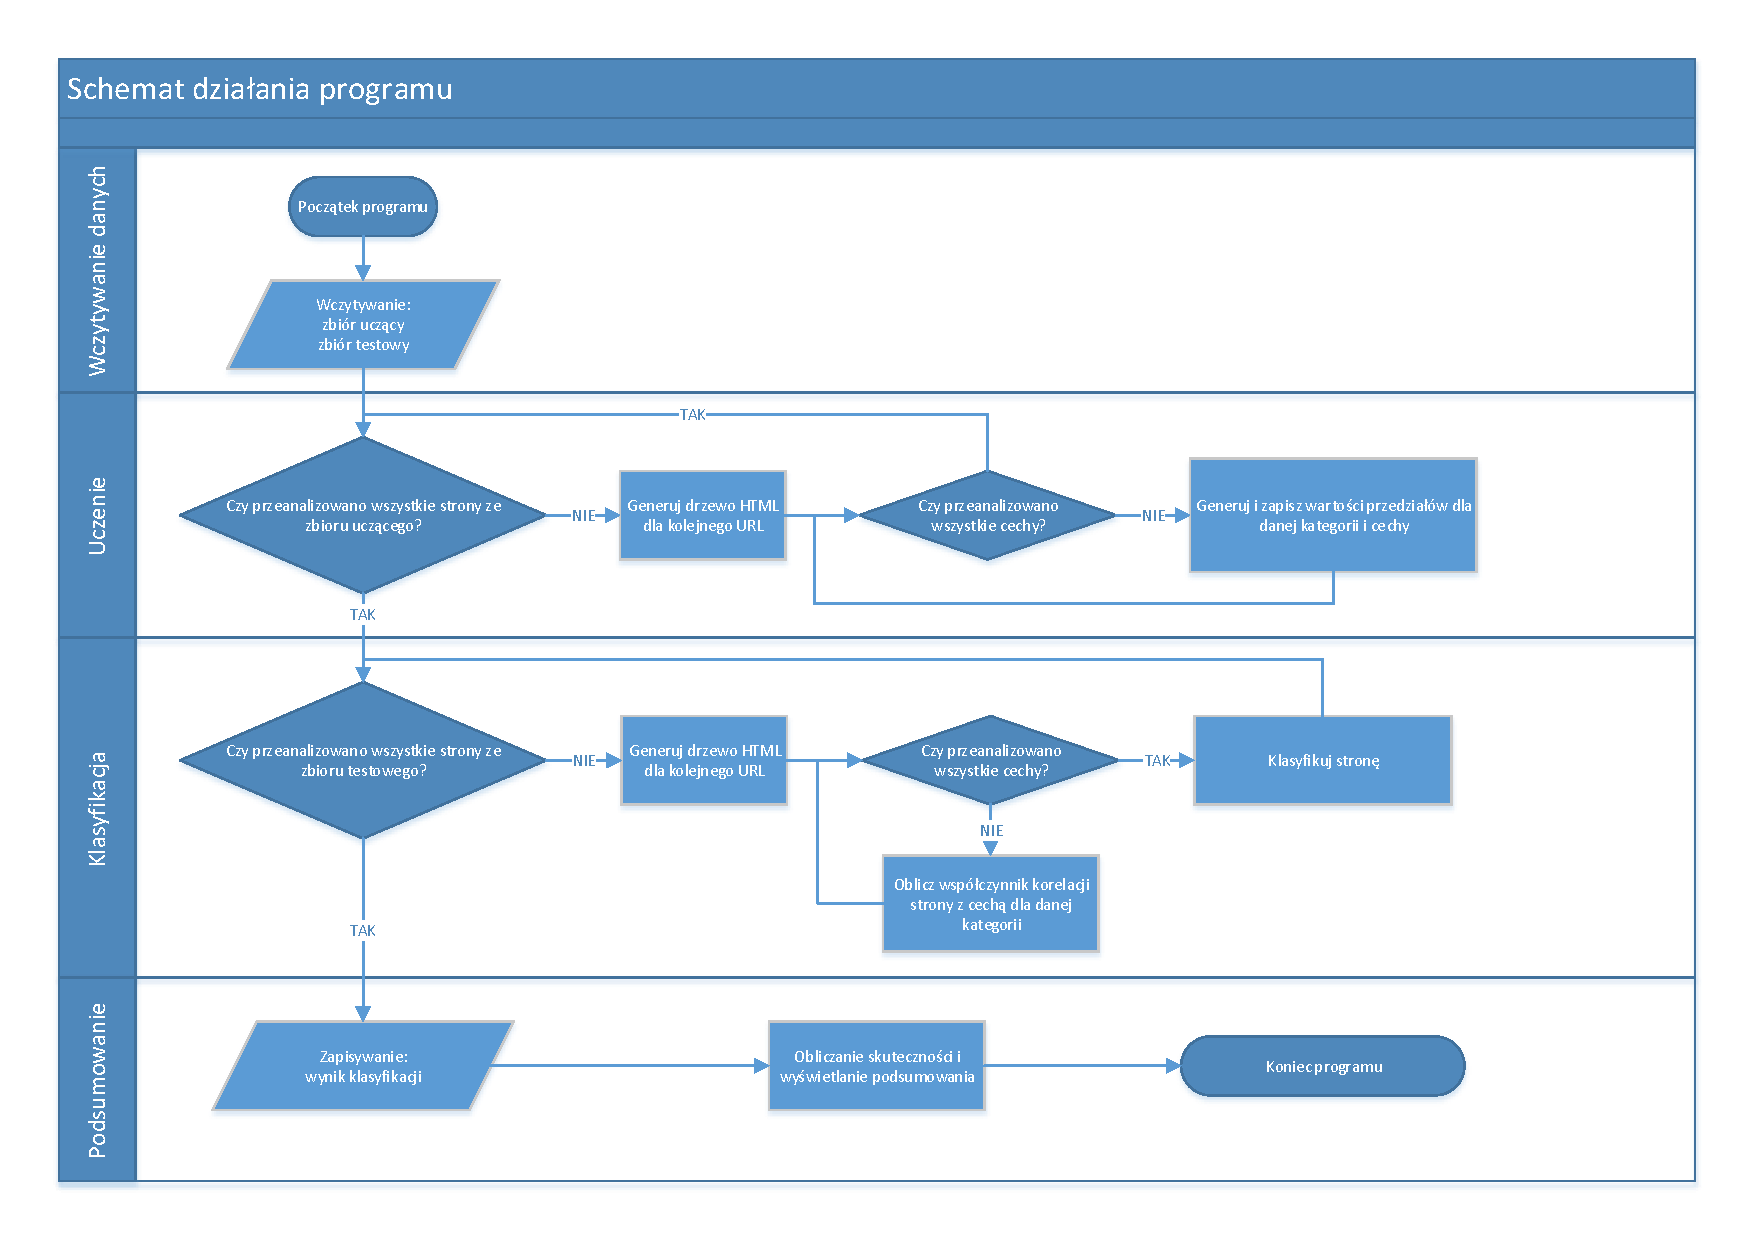
\includepdf[angle=90]{program_schema.pdf}

\subsection{Drzewo HTML}

Strony WWW są wewnętrznie reprezentowane przez drzewo HTML. Każdy korzeń drzewa posiada następujące atrybuty:

\begin{itemize}
    \item tag,
    \item słownik atrybutów (np. \verb+class="main-img", src="image.jpg"+),
    \item tekst wewnątrz taga,
    \item wysokość elementu,
    \item szerokość elementu.
\end{itemize}

Ponadto od dowolnego korzenia można dojść do jego rodzica, a~także wszystkich jego dzieci. Rysunek \ref{fig:html_tree} przedstawia schemat wykorzystywanego drzewa HTML.

\begin{figure}[ht!]
\centering
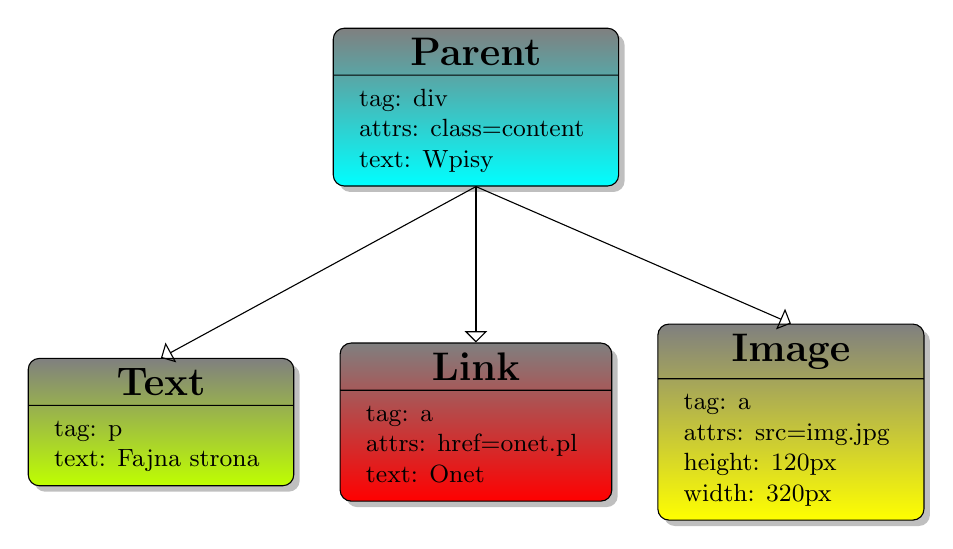
\begin{tikzpicture}[node distance=4cm]
    \node (Parent) [draw=black, rectangle split, rectangle split parts=2, rounded corners, top color=gray, bottom color=cyan, drop shadow]
    {
        {\Large\textbf{Parent}}
        \nodepart{second}
        {\small
        \begin{tabular}{l}
        tag: div \\
        attrs: class=content \\
        text: Wpisy
        \end{tabular}
        }
    };
    \node (Link) [draw=black, rectangle split, rectangle split parts=2, rounded corners, top color=gray, bottom color=red, drop shadow, below of=Parent]
    {
        {\Large\textbf{Link}}
        \nodepart{second}
        {\small
        \begin{tabular}{l}
        tag: a \\
        attrs: href=onet.pl \\
        text: Onet
        \end{tabular}
        }
    };
    \node (Text) [draw=black, rectangle split, rectangle split parts=2, rounded corners, top color=gray, bottom color=lime, drop shadow, left of=Link]
    {
        {\Large\textbf{Text}}
        \nodepart{second}
        {\small
        \begin{tabular}{l}
        tag: p \\
        text: Fajna strona
        \end{tabular}
        }
    };
    \node (Image) [draw=black, rectangle split, rectangle split parts=2, rounded corners, top color=gray, bottom color=yellow, drop shadow, right of=Link]
    {
        {\Large\textbf{Image}}
        \nodepart{second}
        {\small
        \begin{tabular}{l}
        tag: a \\
        attrs: src=img.jpg \\
        height: 120px \\
        width: 320px \\
        \end{tabular}
        }
    };
    \draw[->, >=open triangle 90]   (Parent.south) -- (Image.north);
    \draw[->, >=open triangle 90]   (Parent.south) -- (Text.north);
    \draw[->, >=open triangle 90]   (Parent.south) -- (Link.north);
\end{tikzpicture}
    \caption{Poglądowy schemat drzewa HTML.}
    \label{fig:html_tree}
\end{figure}

Etap budowy drzewa jest w~pełni konfigurowalny, dzięki użyciu następujących atrybutów:

\begin{description}
    \item[dozwolone tagi] Lista tagów, z~których mogą powstawać liście drzewa. Jeżeli tag nie znajduje się na dozwolonej liście, tekst znajdujacy się w~jego środku jest konkatenowany z~tekstem jego pierwszego dozwolonego rodzica.
    \item[dozwolone atrybuty] Lista atrybutów, które są włączane do słownika w~liściach drzewa. Pozostałe atrybuty i~ich wartości są pomijane.
    \item[zakazane tagi] Lista tagów, które zawierają tekst nie włączany do pierwszego dozwolonego rodzica. Umożliwia to odfiltrowywanie m.in. skryptów.
\end{description}

Do budowy drzewa została wykorzystana wewnętrzna biblioteka języka Python - \verb+HTMLParser+\footnote{Dokumentacja biblioteki jest dostępna pod \href{http://docs.python.org/2/library/htmlparser.html}{tym adresem}.}.

\subsection{Główna struktura strony}
\label{sec:main_structure}

Przed omówieniem zestawu cech badanych przez aplikację, należy wprowadzić pojęcie \emph{głównej struktury strony}, która będzie intensywnie analizowana. Główna struktura strony to najliczniejsza struktura, która posiada następujące cechy:

\begin{itemize}
    \item Występują w~niej wyłącznie tagi \verb+<td>+ lub \verb+<div>+, przy czym w~danej strukturze są to tagi wyłącznie jednego z~tych typów.
    \item Wszystkie tagi występują na jednym poziomie głębokości w~drzewie. Oznacza to, że mają wspólnego rodzica.
    \item Każdy z~tagów posiada jednakową wartość atrybutu \verb+class+.
    \item Każdy element struktury posiada więcej niż jeden element podrzędny lub większy niż jeden poziom zagłębienia elementów.
\end{itemize}

Główna struktura jest zaprezentowana na rysunku \ref{fig:structure}.

\begin{figure}[ht!]
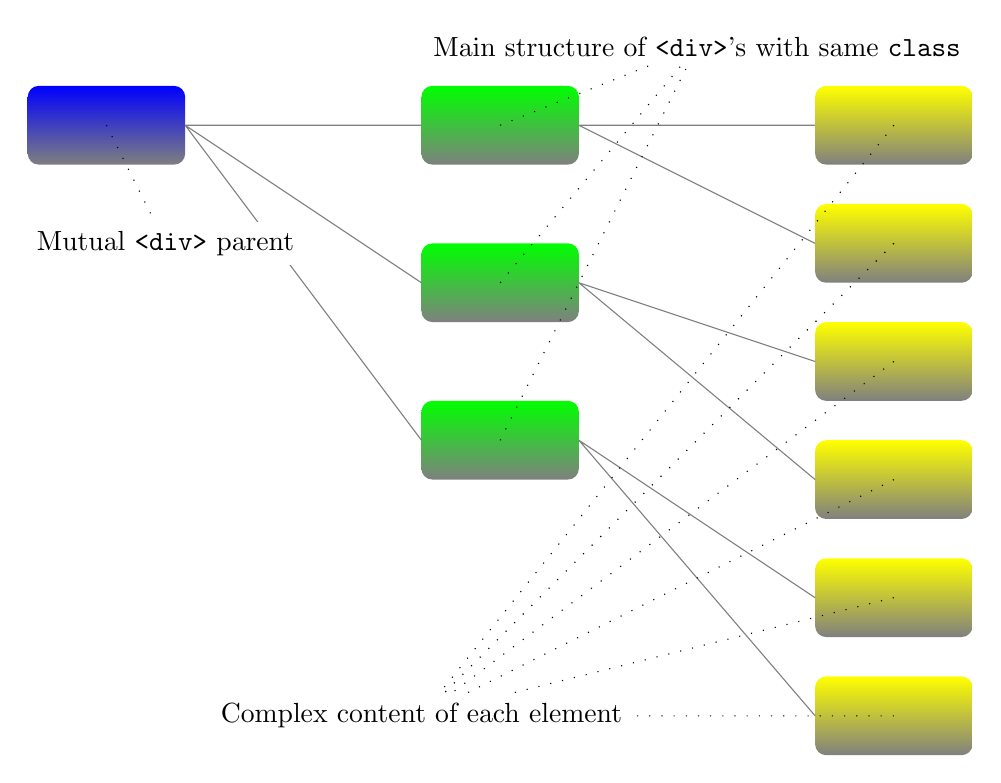
\begin{tikzpicture}
    \shade[rounded corners, top color=blue,bottom color=gray] (0,-1) rectangle (2,0);
    \shade[rounded corners, top color=green,bottom color=gray] (5,0) rectangle (7,-1);
    \shade[rounded corners, top color=green,bottom color=gray] (5,-2) rectangle (7,-3);    
    \shade[rounded corners, top color=green,bottom color=gray] (5,-4) rectangle (7,-5);       
    \shade[rounded corners, top color=yellow,bottom color=gray] (10,0) rectangle (12,-1);
    \shade[rounded corners, top color=yellow,bottom color=gray] (10,-1.5) rectangle (12,-2.5);    
    \shade[rounded corners, top color=yellow,bottom color=gray] (10,-3) rectangle (12,-4);    
    \shade[rounded corners, top color=yellow,bottom color=gray] (10,-4.5) rectangle (12,-5.5);    
    \shade[rounded corners, top color=yellow,bottom color=gray] (10,-6) rectangle (12,-7);    
    \shade[rounded corners, top color=yellow,bottom color=gray] (10,-7.5) rectangle (12,-8.5); 
    
    \draw[draw=gray]
        (2,-0.5) -- (5, -0.5)
        (2,-0.5) -- (5, -2.5)        
        (2,-0.5) -- (5, -4.5)
        (7,-0.5) -- (10, -0.5)
        (7,-0.5) -- (10, -2)
        (7,-2.5) -- (10, -3.5)
        (7,-2.5) -- (10, -5)
        (7,-4.5) -- (10, -6.5)
        (7,-4.5) -- (10, -8);
    \draw[loosely dotted] (1,-0.5) -- (1.75,-2) node[fill=white]
                        {Mutual \verb!<div>! parent};
    \draw[loosely dotted]
        (6, -0.5) -- (8.5,0.5)
        (6, -2.5) -- (8.5,0.5)
        (6, -4.5) -- (8.5,0.5) node[fill=white]
                        {Main structure of \verb!<div>!'s with same \verb!class!}; 
    \draw[loosely dotted]
        (11,-0.5) -- (5, -8)
        (11,-2) -- (5, -8)
        (11,-3.5) -- (5, -8)
        (11,-5) -- (5, -8)
        (11,-6.5) -- (5, -8)
        (11,-8) -- (5, -8) node[fill=white]
                        {Complex content of each element};
\end{tikzpicture}
    \caption{Zielone elementy należą do głównej struktury strony.}
    \label{fig:structure}
\end{figure}

Struktura ta jest charakterystyczna dla wszystkich czterech typów klasyfikowanych stron. Na \emph{blogach} zawiera treść wpisów, na \emph{kwejkach} obrazki, na stronach informacyjnych odnośniki do artykułów, natomiast w~sklepach internetowych - odnośniki do kategorii i/lub produktów.

\subsection{Analizowane cechy strony}

Na etapie uczenia się oraz klasyfikacji brane są pod uwagę, między innymi, następujące cechy:

\begin{itemize}
    \item Liczba elementów w~głównej strukturze strony.
    \item Liczba powtórzeń głównej struktury strony. Sprawdza czy struktura się powtarza i, jeżeli tak, to w~jakiej liczbie.
    \item Średnia ilość tekstu przypadająca na każdy element głównej struktury strony oraz jego dzieci. 
    \item Średnia ilość obrazów przypadająca na każdy element głównej struktury strony oraz jego dzieci.
    \item Liczba obrazów na stronie.
    \item Rozmiary największego oraz najmniejszego obrazu na stronie.
    \item Liczba odnośników na stronie.
    \item Stosunek długości tekstu zawartego w~odnośnikach do długości całego tekstu zawartego na stronie.
    \item Średnia długość lokalnego odnośnika\footnote{Odnośnik lokalny prowadzi do tej samej domeny, w~której znajduje się analizowana strona.} na stronie.
    \item Liczba tagów w~specyfikacji HTML5 (przykładowo: \verb+<article>+ oraz \verb+<section>+).
    \item Stosunek liczby odnośników do liczby obrazów na stronie.
    \item Stosunek długości tekstu do liczby obrazów na stronie.
\end{itemize}

Cechy te dobrze różnicują cztery zadane kategorie stron internetowych. Przykładowo serwisy informacyjne charakteryzują się wysokim współczynnikiem długości tekstu w~odnośnikach do całkowitej długości tekstów, długimi odnośnikami lokalnymi, dużą ilością obrazów na stronie oraz częstym występowaniem tagów w~specyfikacji HTML5. Dla kontrastu blogi charakteryzują się niewielkim stosunkiem liczby odnośników do długości tekstu, niewielką liczbą obrazków, dużą koncentracją tekstu w~głównej strukturze oraz większą niż dla serwisów informacyjnych liczbą elementów w~głównej strukturze strony.

\section{Dane}

Dane wejściowe/wyjściowe są umieszczane w~plikach o~strukturze wewnętrznej \verb+<adres URL>_<kategoria>+. Kolejne dokumenty są rozdzielone znakami nowej linii. Przykład struktury został zaprezentowany poniżej:

\begin{figure}[ht!]
    \begin{Verbatim}[frame=single]
    http://kwejk.pl kwejk
    http://atakklonow.pl kwejk
    http://rafalstec.blox.pl blog
    http://webitect.net blog
    http://onet.pl serwis informacyjny
    http://wp.pl serwis informacyjny
    http://wicomp.pl sklep internetowy
    http://morele.net sklep internetowy
    \end{Verbatim}
    \caption{Struktura danych wejściowych/wyjściowych.}
    \label{fig:input_output_structure}
\end{figure}

\subsection{Dane wejściowe}

Dane wejściowe składają się z~dwóch plików\footnote{Nazwy plików są konfigurowalne, podobnie jak inne ustawienia aplikacji, w~pliku config.ini.}:

\begin{description}
    \item[input\_classified.txt] Dane trenujące dla algorytmu. Na ich podstawie budowana jest lista kategorii stron rozpoznawanych przez system.
    \item[input\_unclassified.txt] Dane testowe dla algorytmu. Strony umieszczone na liście poddawane są klasyfikacji na podstawie wartości parametrów wyznaczonych przez dane trenujące. Wstępna klasyfikacja stron jest niezbędna do obliczenia skuteczności algorytmu i~nie jest brana pod uwagę przez właściwy algorytm.
\end{description}

\subsection{Dane wyjściowe}

Na dane wyjściowe składają się zarówno pliki, jak również wyjście standardowe (konsola):

\begin{description}
    \item[plik output.txt] Wynik działania algorytmu. Zawiera adresy analizowanych stron i~przyporządkowaną im przez algorytm klasyfikację.
    \item[wynik konfiguracji] Wyprowadzany na wyjście standardowe. Przedstawia wartości dozwolonych przedziałów cech, w~ramach kategorii, wyznaczone na podstawie danych testowych.
    \item[podsumowanie] Wyprowadzane na wyjście standardowe. Przedstawia skuteczności algorytmu dla każdej kategorii, mierzone w~czterech własnościach:
        \begin{itemize}
            \item dokładność,
            \item zupełność,
            \item zaszumienie,
            \item precyzja.
        \end{itemize}
\end{description}

\section{Skuteczność algorytmu}

Skuteczność algorytmu mierzona jest przy pomocy czterech wskaźników. Zakładając, że:
 
\begin{itemize}
 \item $|TP|$ to liczba poprawnych przydzieleń dokumentu do danej kategorii, 
 \item $|FP|$ to liczba niepoprawnych przydzieleń dokumentu do danej kategorii,
 \item $|TN|$ to liczba poprawnych nieprzydzieleń dokumentu do danej kategorii,
 \item $|FN|$ to liczba niepoprawnych nieprzydzieleń dokumentu do danej kategorii,
\end{itemize}

wtedy wskaźniki te wyrażają się następującymi wzorami:

\begin{description}
    \item[dokładność] $\frac{|TP| + |TN|}{|TP| + |TN| + |FP| + |FN|}$,
    \item[zupełność] $\frac{|TP|}{|TP| + |FN|}$,
    \item[zaszumienie] $\frac{|FP|}{|FP| + |TN|}$,
    \item[precyzja] $\frac{|TP|}{|TP| + |FP|}$.
\end{description}

Wskaźniki te można odczytywać następująco:

\begin{description}
    \item[dokładność] opisuje procent poprawnych wskazań algorytmu ogółem.
    \item[zupełność] opisuje procent pokrycia wejściowego zbioru danych poprawnymi wskazaniami.
    \item[zaszumienie] opisuje procent właściwości wskazań negatywnych.
    \item[precyzja] opisuje procent właściwości wskazań pozytywnych.
\end{description}

\subsection{Okrojone dane testowe}

Tabela \ref{tab:reduced_set_accuracy} przedstawia wynik działania algorytmu dla okrojonych danych testowych, przygotowanych na potrzeby prezentacji. Okrojone dane testowe obejmują:

\begin{itemize}
    \item po trzy przykłady trenujące z~każdej z~czterech kategorii,
    \item po dziesięć przykładów stron do sklasyfikowania z~każdej z~czterech kategorii,
    \item pięć stron, które nie należą do żadnej z~czterech kategorii.
\end{itemize}

\begin{table}[ht!]
\centering
    \begin{tabular}{| c | c | c | c | c | c |}
        \hline
        \multicolumn{2}{|c|}{} & \multicolumn{4}{c|}{Wskaźniki} \\
        \cline{3-6}
        \multicolumn{2}{|c|}{} & Dokładność & Szczegółowość & Rozrzut & Precyzja \\
        \hline
        \multirow{6}{*}{\begin{sideways}Kategorie \end{sideways}} & Blogi & 98\% & 100\% & 3\% & 91\% \\
        \cline{2-6}
        & Kwejki & 95\% & 100\% & 6\% & 83\% \\
        \cline{2-6}
        & Serwisy & \multirow{2}{*}{93\%} & \multirow{2}{*}{88\%} & \multirow{2}{*}{6\%} & \multirow{2}{*}{78\%} \\
        & informacyjne & & & & \\
        \cline{2-6}
        & Sklepy & \multirow{2}{*}{93\%} & \multirow{2}{*}{70\%} & \multirow{2}{*}{0\%} & \multirow{2}{*}{100\%} \\
        & internetowe & & & & \\
        \hline
    \end{tabular}
    \caption{Skuteczność algorytmu dla okrojonego zestawu danych testowych.}
    \label{tab:reduced_set_accuracy}
\end{table}

Widać, że zaimplementowany algorytm zapewnia bardzo wysoką skuteczność. Wyróżnia się zwłaszcza skuteczność klasyfikacji blogów, dla której najgorszy z~wymienionych wskaźników ma rozrzut $\pm 9\%$ względem doskonałości. Licząc średnie odchylenie wskaźników od doskonałości można wywnioskować, że  algorytm jest miarodajny w~$92,125\%$ przypadków.

\end{document}